\begin{figure}[H]
\centering
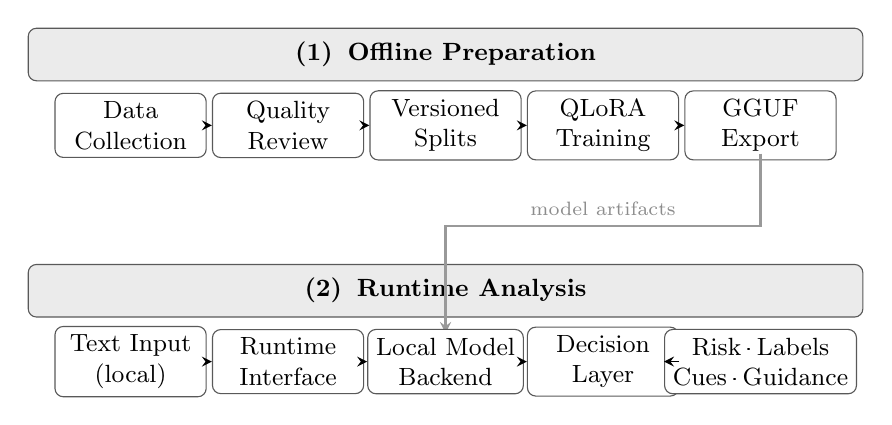
\begin{tikzpicture}[
  box/.style={
    draw=black!65, fill=white, rectangle, rounded corners=3pt,
    minimum width=1.92cm, minimum height=0.72cm,
    align=center, font=\small, inner sep=3pt
  },
  hdr/.style={
    draw=black!65, fill=black!8, rectangle, rounded corners=3pt,
    minimum width=10.6cm, minimum height=0.46cm,
    align=left, font=\small\bfseries, inner sep=5pt
  },
  arr/.style={->, >=stealth, semithick},
  darr/.style={->, >=stealth, thick, black!40}
]

%% ── Section headers ──────────────────────────────────────────
\node[hdr] at (0,  0.00) {\small (1)\enspace Offline Preparation};
\node[hdr] at (0, -3.00) {\small (2)\enspace Runtime Analysis};

%% ── Offline row ──────────────────────────────────────────────
\node[box] (dc)  at (-4.0, -0.90) {Data\\Collection};
\node[box] (qrv) at (-2.0, -0.90) {Quality\\Review};
\node[box] (spl) at ( 0.0, -0.90) {Versioned\\Splits};
\node[box] (qlo) at ( 2.0, -0.90) {QLoRA\\Training};
\node[box] (gex) at ( 4.0, -0.90) {GGUF\\Export};

\draw[arr] (dc)  -- (qrv);
\draw[arr] (qrv) -- (spl);
\draw[arr] (spl) -- (qlo);
\draw[arr] (qlo) -- (gex);

%% ── Model artifact handoff (dashed, GGUF → Local Model) ──────
\draw[darr]
  (4.0, -1.26) -- (4.0, -2.18)
  -- node[above, font=\scriptsize, text=black!45] {model artifacts}
  (0.0, -2.18)
  -- (0.0, -3.54);

%% ── Runtime row ──────────────────────────────────────────────
\node[box] (inp) at (-4.0, -3.90) {Text Input\\(local)};
\node[box] (rif) at (-2.0, -3.90) {Runtime\\Interface};
\node[box] (mod) at ( 0.0, -3.90) {Local Model\\Backend};
\node[box] (dly) at ( 2.0, -3.90) {Decision\\Layer};
\node[box, minimum width=2.15cm] (out) at ( 4.0, -3.90)
  {Risk\,·\,Labels\\Cues\,·\,Guidance};

\draw[arr] (inp) -- (rif);
\draw[arr] (rif) -- (mod);
\draw[arr] (mod) -- (dly);
\draw[arr] (dly) -- (out);

\end{tikzpicture}
\caption{End-to-end system overview: dataset pipeline, local runtime, model deployment profiles, and explainable decision layer.}
\label{fig:system-overview}
\end{figure}
